\subsection{Decision Trees}
\label{decision_trees}

\noindent{\bf Description}
Decision trees (for classification) is a classifier that is considered
more interpretable than other statistical classifiers. This implementation
is well-suited to handle large-scale data and builds a (binary) decision 
tree in parallel.\\

\noindent{\bf Usage}
\begin{tabbing}
\texttt{-f} \textit{path}/\texttt{decision-tree.dml -nvargs} 
\=\texttt{X=}\textit{path}/\textit{file} 
  \texttt{Y=}\textit{path}/\textit{file} 
  \texttt{types=}\textit{path}/\textit{file}\\
\>\texttt{model=}\textit{path}/\textit{file}
  \texttt{bins=}\textit{int}
  \texttt{depth=}\textit{int}\\
\>\texttt{num\_leaf=}\textit{int}
  \texttt{num\_samples=}\textit{int}\\
\>\texttt{Log=}\textit{path}/\textit{file}
  \texttt{fmt=}\textit{csv}$\vert$\textit{text}
\end{tabbing}

\begin{tabbing}
\texttt{-f} \textit{path}/\texttt{decision-tree-predict.dml -nvargs} 
\=\texttt{X=}\textit{path}/\textit{file} 
  \texttt{Y=}\textit{path}/\textit{file} 
  \texttt{model=}\textit{path}/\textit{file}\\
\>\texttt{fmt=}\textit{csv}$\vert$\textit{text}
  \texttt{accuracy=}\textit{path}/\textit{file}\\
\>\texttt{confusion=}\textit{path}/\textit{file}
  \texttt{predictions=}\textit{path}/\textit{file}
\end{tabbing}

\noindent{\bf Arguments}

\begin{itemize}
\item X: Location (on HDFS) to read the matrix of feature vectors; 
each row constitutes one feature vector.
\item Y: Location (on HDFS) to read the one-column matrix of (categorical) 
labels that correspond to feature vectors in X. Classes are assumed to be
contiguously labeled beginning from 1. Note that, this argument is optional
for prediction.
\item model: Location (on HDFS) that contains the learnt decision tree.
\item types: Location (on HDFS) that contains each feature's type. 1 denotes
continuous-valued (scale) and 2 denotes categorical.
\item bins (default: {\tt 50}): Number of thresholds to choose for each 
continuous-valued feature (deterimined by equi-height binning). 
\item depth (default: {\tt 10}): Maximum depth of the learnt decision tree.
\item num\_leaf (default: {\tt 1}): Parameter that controls pruning. The tree
is not expanded if a node receives less than num\_leaf training examples.
\item num\_samples (default: {\tt 10}): Parameter that decides when to switch
to in-memory building of subtrees. If a node $v$ receives less than num\_samples
training examples then this implementation switches to an in-memory subtree
building procedure to build the subtree under $v$ in its entirety.
\item Log: Location (on HDFS) that collects various useful metrics that indicate
training progress.
\item predictions: Location (on HDFS) to store predictions for a held-out test set.
Note that, this is an optional argument.
\item fmt (default: {\tt text}): Specifies the output format. Choice of 
comma-separated values (csv) or as a sparse-matrix (text).
\item accuracy: Location (on HDFS) to store the testing accuracy from a 
held-out test set during prediction. Note that, this is an optional argument.
\item confusion: Location (on HDFS) to store the confusion matrix
computed using a held-out test set. Note that, this is an optional 
argument.
\end{itemize}

\noindent{\bf Details}
 
Decision trees (Breiman et al, 1984) are simple models of
classification that,  due to their structure,  are easy to
interpret. Given an example feature vector, each node in the learnt
tree runs a simple test on it. Based on the result of the test, the
example is either diverted to the left subtree or to the right
subtree. Once the example reaches a leaf, then the label stored at the
leaf is returned as the prediction for the example.

\par

Building a decision tree from a fully labeled training set entails
choosing appropriate tests for each internal node in the tree and this
is usually performed in a top-down manner. Choosing a test requires
first choosing a feature $j$ and depending on the type of $j$, either
a threshold $\sigma$, in case $j$ is continuous-valued, or a subset of
values $S \subseteq \text{Dom}(j)$ where $\text{Dom}(j)$ denotes
domain of $j$, in case it is categorical. For continuous-valued
features the test is thus of form $x_j < \sigma$ and for categorical
features it is of form $x_j \in S$, where $x_j$ denotes the $j^{th}$
feature value of feature vector $x$. One way to determine which test
to include, is to compare impurities of the subtrees induced by the
test and this implementation uses {\it Gini impurity}.

\par

The current implementation allows the user to specify the maximum
depth of the learnt tree using the argument {\it depth}. It also
allows for some automated pruning via the argument {\it num\_leaf}. If
a node receives $\leq$ {\it num\_leaf} training examples, then a leaf
is built in its place. Furthermore, for a continuous-valued feature
$j$ the number of candidate thresholds $\sigma$ to choose from is of
the order of the number of examples present in the training set. Since
for large-scale data this can result in a large number of candidate
thresholds, the user can limit this number via the arguments {\it
  bins} which controls the number of candidate thresholds considered
for each continuous-valued feature. For each continuous-valued
feature, the implementation computes an equi-height histogram to
generate one candidate threshold per equi-height bin. To determine the
best value subset to split on in the case of categorical features,
this implementation greedily includes values from the feature's domain
until the sum of the impurities of the subtrees induced stops
improving.

\par

Learning a decision tree on large-scale data has received  some
attention in the literature. The current implementation includes logic
for choosing tests for multiple nodes that belong to the same level in
the decision tree in parallel (breadth-first expansion) and for
building entire subtrees under multiple nodes in parallel (depth-first
subtree building). Empirically it has been demonstrated that it is
advantageous to perform breadth-first expansion for the nodes
belonging to the top levels of the tree and to perform depth-first
subtree building for nodes belonging to the lower levels of the tree
(Panda et al, 2009). The parameter {\it num\_samples} controls when we
switch to  depth-first subtree building. Any node in the decision tree
that receives $\leq$ {\it num\_samples} training examples, the subtree
under it is built in its entirety in one shot.

\par

{\it Description of the model}: The learnt decision tree is represented using a matrix that
contains at least 3 rows. Each column in the matrix contains the parameters relevant
to a single node in the tree. The $i^{th}$ column denotes the parameters for the $i^{th}$ node
whose left child is stored in the $2i^{th}$ column and right child is stored in the $2i+1^{th}$
column. Here is a brief description of what each row in the matrix contains:
\begin{itemize}
\item $1^{st}$ row: Contains the feature index of the feature that this node looks at if 
the node is an internal node, otherwise -1.
\item $2^{nd}$ row: Contains the type of the feature that this node looks at if the node is
an internal node, otherwise the label this leaf node is supposed to predict. 
1 denotes continuous-valued feature and 2 denotes categorical.
\item $3^{rd}$: Only applicable for internal nodes. Contains the threshold the example's 
feature value is compared to if the feature chosen for this node is a continuous-valued feature. 
If on the other hand, the feature chosen for this node is categorical then the size of the 
subset of values is stored here.
\item $4^{th}$ row onwards: Only applicable in the case of internal nodes where the feature
chosen is a categorical feature. Rows $4, 5 \ldots$ depict the value subset 
chosen for this node.
\end{itemize}
As an example, Figure \ref{dtree} shows a decision tree with $5$ nodes and its matrix
representation.

\begin{figure}
\begin{minipage}{0.3\linewidth}
\begin{center}
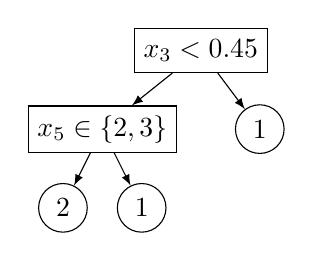
\begin{tikzpicture}
\node (labelleft) [draw,shape=circle,minimum size=16pt] at (0,0) {$2$};
\node (labelright) [draw,shape=circle,minimum size=16pt] at (1,0) {$1$};
\node (rootleft) [draw,shape=rectangle,minimum size=16pt] at (0.5,1) {$x_5 \in \{2,3\}$};
\node (rootlabel) [draw,shape=circle,minimum size=16pt] at (2.5,1) {$1$};
\node (root) [draw,shape=rectangle,minimum size=16pt] at (1.75,2) {$x_3 < 0.45$};

\draw[-latex] (root) -- (rootleft);
\draw[-latex] (root) -- (rootlabel);
\draw[-latex] (rootleft) -- (labelleft);
\draw[-latex] (rootleft) -- (labelright);

\end{tikzpicture}
\end{center}
\begin{center}
(a)
\end{center}
\end{minipage}
\hfill
\begin{minipage}{0.65\linewidth}
\begin{center}
\begin{tabular}{c|c|c|c|c|c|}
& Col 1 & Col 2 & Col 3 & Col 4 & Col 5\\
\hline
Row 1 & 3 & 5 & -1 & -1 & -1\\
\hline
Row 2 & 1 & 2 & 1 & 2 & 1\\
\hline
Row 3 & 0.45 & 2 &  &  & \\
\hline
Row 4 &  & 2 &  &  & \\
\hline
Row 5 &  & 3 &  &  & \\
\hline
\end{tabular}
\end{center}
\begin{center}
(b)
\end{center}
\end{minipage}
\caption{(a) An example tree and its (b) matrix representation. $x$ denotes an example and $x_j$ the $j^{th}$ feature's value in it.}
\label{dtree}
\end{figure}

\vspace{16pt}

\noindent{\bf Returns}

The matrix corresponding to the learnt model is written to a file in the format requested. See
details where the structure of the model matrix is
described. Depending on what arguments are provided during
invocation, decision-tree-predict.dml may compute one or more of
predictions,  accuracy and confusion matrix in the requested output format.
\\

\noindent{\bf Examples}
\begin{verbatim}
hadoop jar SystemML.jar -f decision-tree.dml -nvargs 
                           X=/user/biadmin/X.mtx 
                           Y=/user/biadmin/y.mtx 
                           types=/user/biadmin/types.mtx
                           model=/user/biadmin/model.mtx
                           bins=50 depth=10 num_leaf=1
                           num_samples=250 fmt=csv
                           Log=/user/biadmin/accuracy.csv
\end{verbatim}

\begin{verbatim}
hadoop jar SystemML.jar -f decision-tree-predict.dml -nvargs 
                           X=/user/biadmin/X.mtx 
                           Y=/user/biadmin/y.mtx 
                           model=/user/biadmin/model.mtx
                           fmt=csv
                           predictions=/user/biadmin/probabilities.csv
                           accuracy=/user/biadmin/accuracy.csv
                           confusion=/user/biadmin/confusion.csv
\end{verbatim}

\noindent{\bf References}

\begin{itemize}
\item B. Panda, J. Herbach, S. Basu, and R. Bayardo. \newblock{PLANET: massively parallel learning of tree ensembles with MapReduce}. In Proceedings of the VLDB Endowment, 2009.
\item L. Breiman, J. Friedman, R. Olshen, and C. Stone. \newblock{Classification and Regression Trees}. Wadsworth and Brooks, 1984.
\end{itemize}
